\section{Sandbox application}\label{sec:sandbox}
The sandbox (\code{sandbox/app.py}, Streamlit~1.65~\cite{streamlit}) is the single control
surface for someone who did not build the system. It runs as root inside the VM and is
opened in a browser on the host (Mac or Windows) at \url{http://localhost:8501}. Its controls map one-to-one onto the
required capabilities (Table~\ref{tab:sandbox}). Every action goes through
\code{sandbox/testbed.py}. That is the same library the scripted experiments use, so a result
seen in the demo can be reproduced exactly by script. Every action is also appended to the
run's \code{events.csv}, which later annotates the plots.

\begin{table}[H]\centering\small
\caption{Sandbox capabilities and how each is realised in the testbed.}\label{tab:sandbox}
\begin{tabularx}{\linewidth}{>{\raggedright}p{3.2cm}>{\raggedright}p{3.6cm}>{\raggedright\arraybackslash}X}
\toprule
Requirement & UI control & Mechanism\\
\midrule
Select a scenario & sidebar: \emph{Service scenario} + \emph{Apply} & preset of per-slice tc parameters + traffic profiles (S1 baseline, S2 factory peak, S3 degraded transport, S4 massive-IoT burst)\\
Bring slices up/down & per-slice \emph{Slice up / Slice down} & switch-off deregistration of the slice's UEs, then re-attach with a runtime config without (or with) that S-NSSAI; multi-slice UEs keep their other session\\
Start/stop traffic per slice & \emph{Start / Stop traffic} & generator processes in the \code{ran} netns bound to the UE's current PDU address (process groups, so stop is clean)\\
Change a slice parameter live & \emph{Live slice parameters} form (MBR, delay, loss) & \code{tc class change} (HTB rate) and \code{tc qdisc change} (netem) on DL tun + UL N6 class; no session impact\\
View live per-slice KPIs & metrics + charts, auto-refresh 2\,s & 1-s KPI rows aggregated per slice: throughput, RTT p50/p99, loss\\
Export run data & \emph{Export run (ZIP)} & KPI CSVs, event log, UE/PDU table, current QoS\\
\bottomrule
\end{tabularx}
\end{table}

\begin{figure}[!htbp]\centering
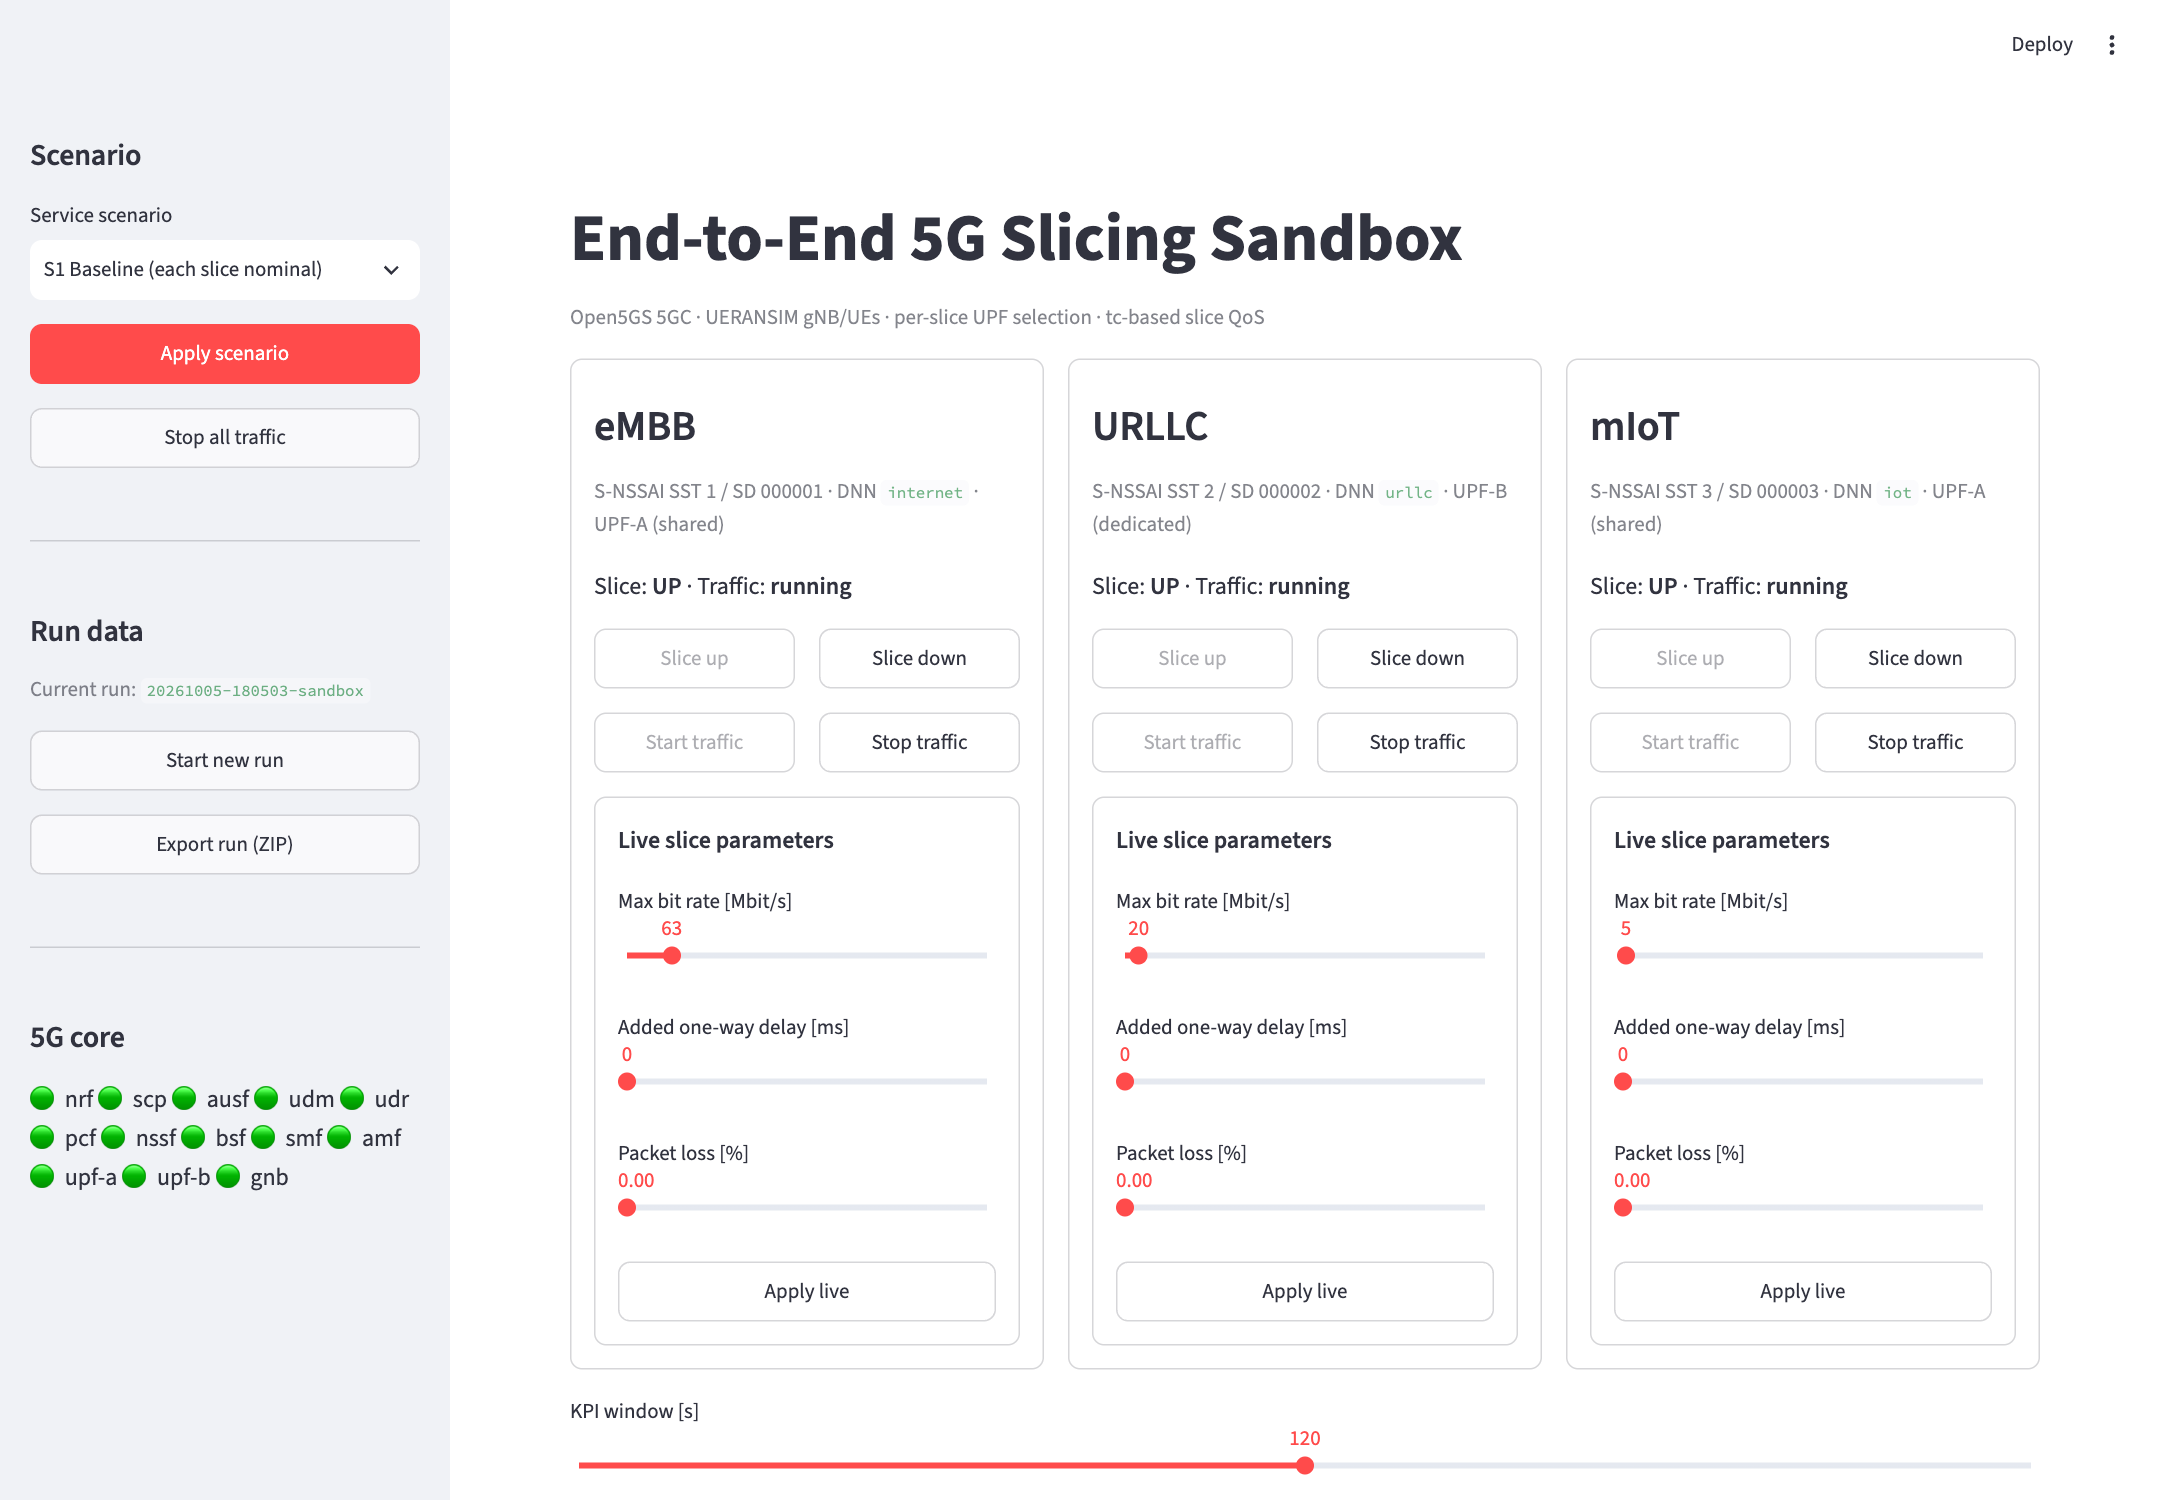
\includegraphics[width=0.86\linewidth]{screenshots/sandbox_top.png}
\caption{Sandbox during scenario S1. Each slice card shows its S-NSSAI, DNN and UPF, its admin
and traffic state, and the live parameter form. The 5GC NF health is shown in the sidebar.}
\label{fig:sandbox1}
\end{figure}
\begin{figure}[!htbp]\centering
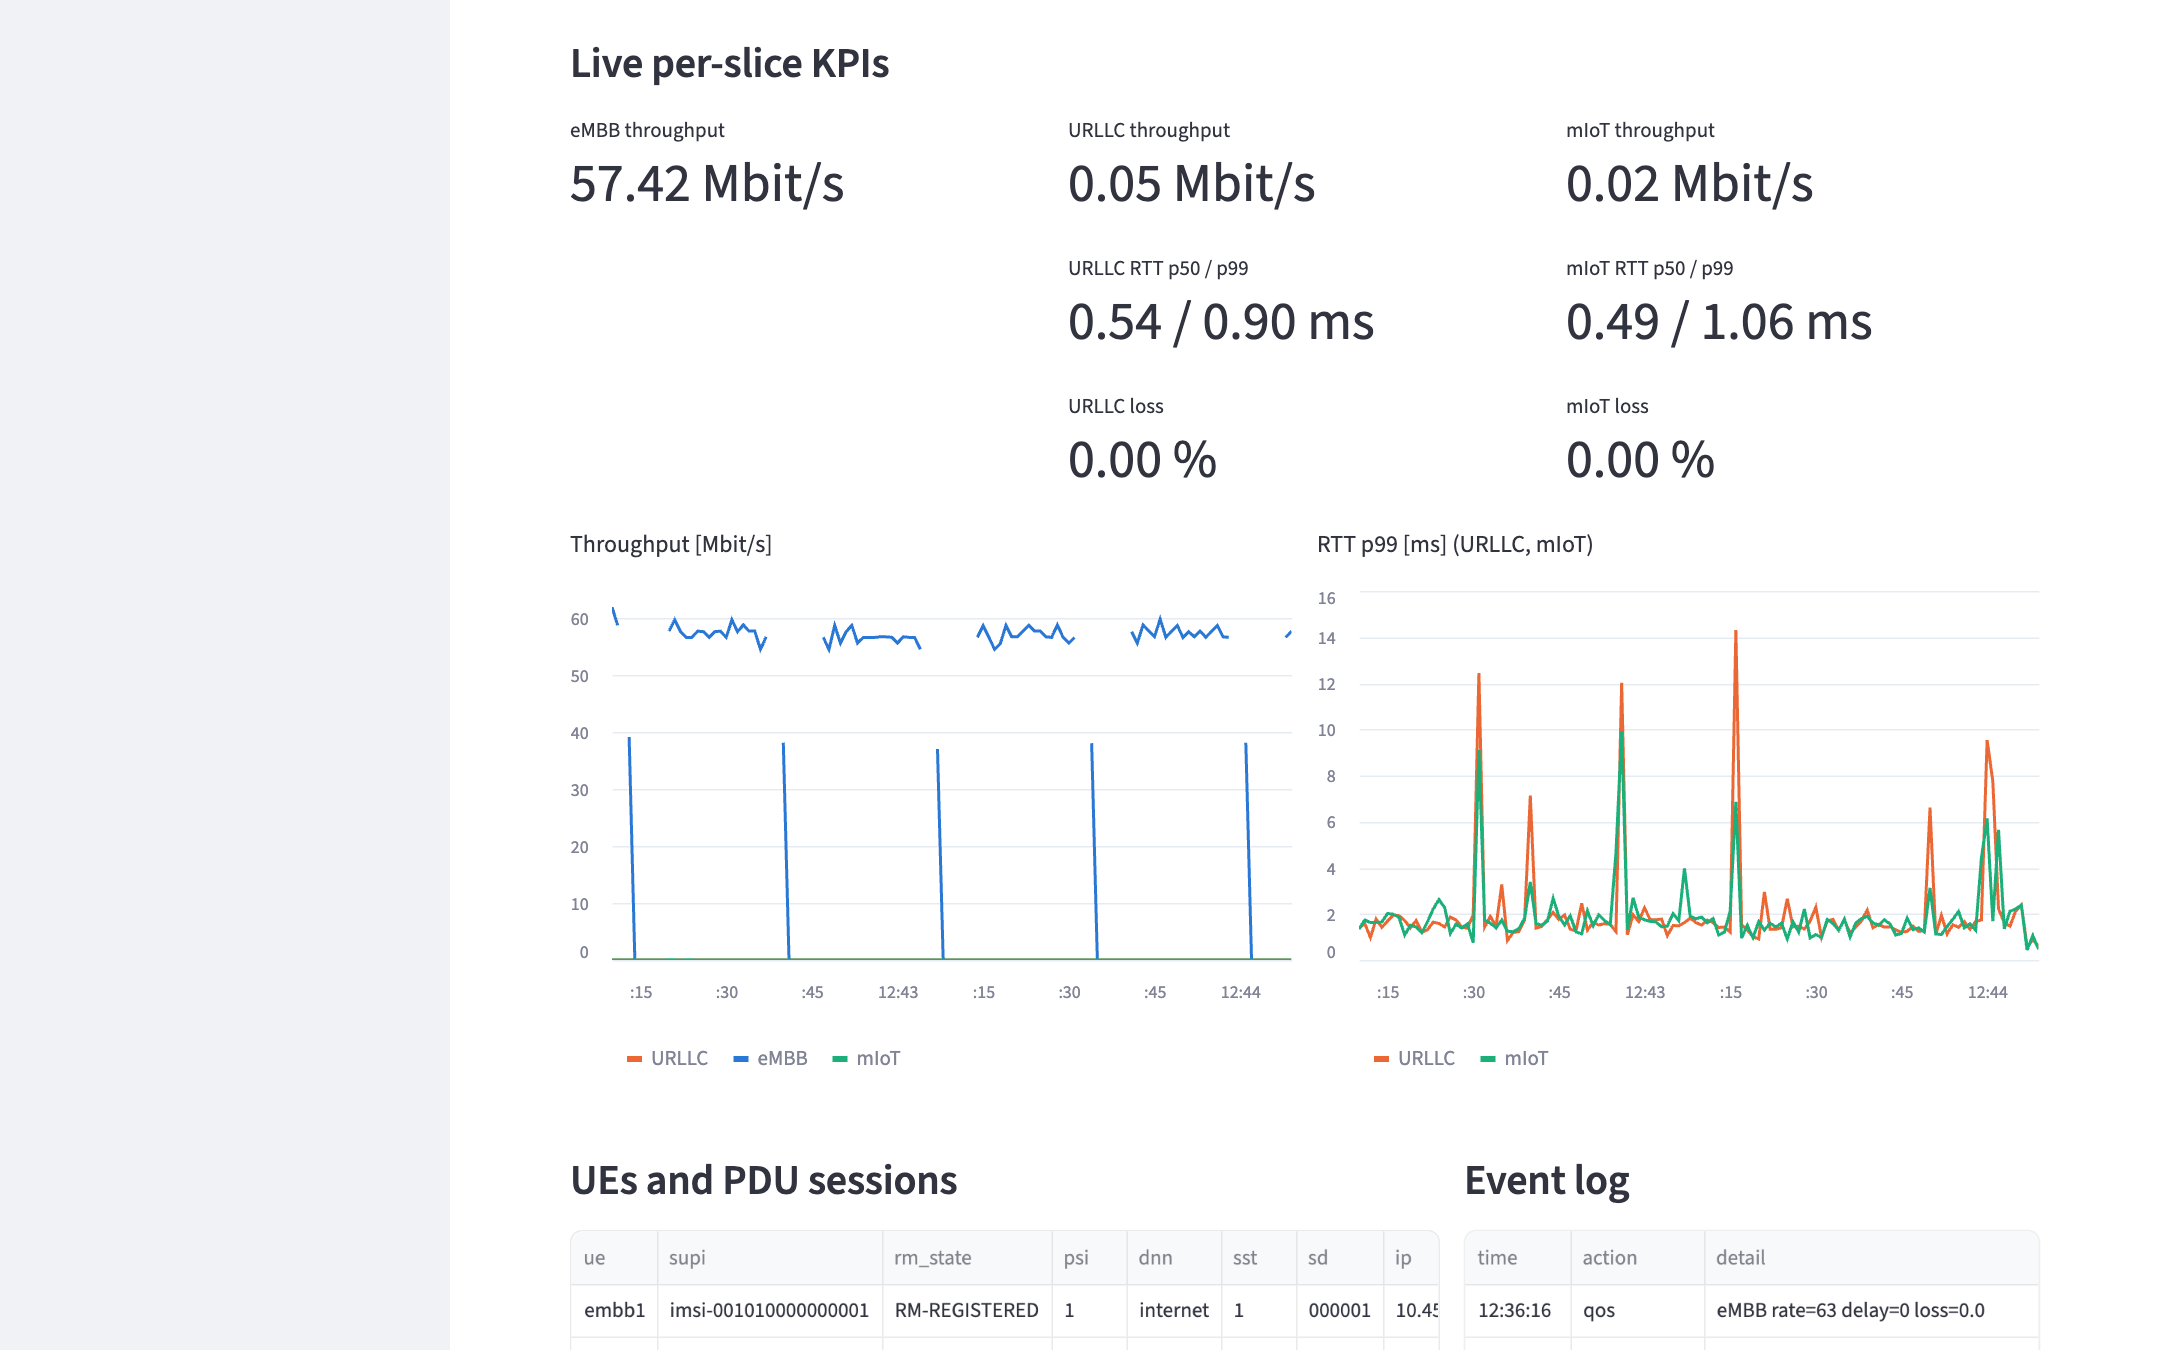
\includegraphics[width=0.86\linewidth]{screenshots/sandbox_kpis.png}
\caption{Sandbox live KPI panel, UE/PDU-session table and event log after a live change of the
eMBB MBR.}\label{fig:sandbox2}
\end{figure}

\paragraph{Design decision: slice down.} Our first implementation released the slice's PDU
sessions with \code{nr-cli ps-release}. UERANSIM, however, re-establishes every session listed
in its config within $\approx$200\,ms, so the slice came straight back (with new addresses).
The final design treats ``slice down'' as an administrative state
(\code{/run/e2e5g/state-<slice>}). The affected UEs perform a switch-off deregistration, which
makes the AMF/SMF release all their contexts and PFCP sessions. They then re-attach from a
runtime config filtered to the slices that are still up. This also exercises the
deregistration and re-registration procedures on demand.
